\documentclass[landscape]{article}
\usepackage[a4paper,margin=3mm,landscape]{geometry}
\usepackage[scaled=0.92]{helvet}
\usepackage{multicol, multirow}
\usepackage{makecell}
\usepackage{array} 
\usepackage[table]{xcolor}
\usepackage{enumitem} 
\usepackage{amssymb}
\usepackage{graphicx}
\setlist{nosep}

\graphicspath{{./images/}}

\pdfinfo{
    /Title (CS2102 Cheatsheet.pdf)
    /Creator (TeX)
    /Producer (pdfTeX 1.40.0)
    /Author (Selwyn Ang)
    /Subject (CS2102)
    /Keywords (CS2102, Cheatsheet, NUS, Database Systems) 
}

% Turn off header and footer
\pagestyle{empty}


\makeatletter
\DeclareRobustCommand\smaller{\@setfontsize\smaller{6pt}{6.5pt}}
\makeatother

% redefine section commands to use less space
\makeatletter
\renewcommand{\section}{\@startsection{section}{1}{0mm}%
  {-0.1ex plus -0.1ex minus -0.1ex}%
  {0.1ex plus .1ex minus 0.1ex}%
{\normalfont\small\bfseries}}
\renewcommand{\subsection}{\@startsection{subsection}{2}{0mm}%
  {-0.1ex plus -0.1ex minus -0.1ex}%
  {0.1ex plus .1ex minus 0.1ex}%
{\normalfont\scriptsize\bfseries}}
\renewcommand{\subsubsection}{\@startsection{subsubsection}{3}{0mm}%
  {-0.1ex plus -0.1ex minus -0.1ex}%
  {0.1ex plus .1ex minus 0.1ex}%
{\normalfont\smaller\bfseries}}%
\makeatother



\renewcommand{\familydefault}{\sfdefault}
\renewcommand\rmdefault{\sfdefault}
%  makes nested numbering (e.g. 1.1.1, 1.1.2, etc)
\renewcommand{\labelenumii}{\theenumii}
\renewcommand{\theenumii}{\theenumi.\arabic{enumii}.}
\renewcommand\labelitemii{•}
\renewcommand\labelitemiii{•}

\setlength{\parindent}{0pt}
\setlength{\parskip}{0pt plus 0.5ex}
\setlength{\columnsep}{0.2cm}
%% adjust spacing for all itemize/enumerate
\setlength{\leftmargini}{0.5cm}
\setlength{\leftmarginii}{0.5cm}
\setlist[itemize,1]{leftmargin=2mm,labelindent=1mm,labelsep=1mm}
\setlist[itemize,2]{leftmargin=2mm,labelindent=1mm,labelsep=1mm}
\setlist[itemize,3]{leftmargin=2mm,labelindent=1mm,labelsep=1mm}
\setlist[enumerate,1]{leftmargin=2mm,labelindent=1mm,labelsep=1mm}
\setlist[enumerate,2]{leftmargin=2mm,labelindent=1mm,labelsep=1mm}
\setlist[enumerate,3]{leftmargin=2mm,labelindent=1mm,labelsep=1mm}

% tightcenter
\newenvironment{tightcenter}{%
  \setlength\topsep{0pt}
  \setlength\parskip{0pt}
  \begin{center}
    }{%
  \end{center}
}

% boxed
\newenvironment{tightbox}{%
  \setlength\topsep{0pt}
  \setlength\parskip{0pt}
  \begin{center}
    \begin{tabular}{|@{\hspace{\dimexpr\fboxsep+0.5\arrayrulewidth}}c@{\hspace{\dimexpr\fboxsep+0.5\arrayrulewidth}}|}
      \hline
    }
    {%
    \\ \hline
    \end{tabular}
  \end{center}
}

% fixed width box
\newenvironment{fixedbox}[1][0.7]{
  \setlength\topsep{0pt}
  \setlength\parskip{0pt}
  \begin{center}
    \begin{tabular}{|>{\centering\arraybackslash}m{#1\linewidth}|}
    \hline
  }{
  \\ \hline
  \end{tabular}
  \end{center}
}

% definition of a new term
\usepackage{soul}
\definecolor{paleyellow}{RGB}{251,243,218}
\newcommand{\definition}[2][]{\sethlcolor{paleyellow}\hl{\textbf{#2}} #1  $\rightarrow$}
% inline definition
\newcommand{\ildefinition}[1]{\sethlcolor{paleyellow}\hl{\textbf{#1}}}

% important note (attention)
\newcommand{\attention}{{\color{red}\textbf{! }}}

% nice proof
\newenvironment{niceproof}[1][Proof]
{%
  \sbox0{\textit{#1}. }%
  \list{}{\labelwidth\wd0 \leftmargin\wd0 \labelsep 0pt }
\item[\usebox0]}
  {\endlist}


\usepackage{color, soul}
\usepackage{listings}
\usepackage{inconsolata}

\definecolor{codegreen}{rgb}{0,0.6,0}
\definecolor{codegray}{rgb}{0.5,0.5,0.5}
\definecolor{codepurple}{HTML}{C42043}
\definecolor{backcolour}{HTML}{F2F2F2}
\definecolor{bookColor}{cmyk}{0,0,0,0.90}

\newcommand{\code}[1]{\texttt{\sethlcolor{backcolour}\hl{$\,$#1$\,$}}}

% SQL code blocks
% define SQL styles
\lstdefinestyle{mySQL}{%
  language=SQL,
  backgroundcolor=\color{backcolour},
  commentstyle=\color{codegreen},
  keywordstyle=\color{codepurple},
  numberstyle=\numberstyle,
  stringstyle=\color{codepurple},
  basicstyle=\scriptsize\ttfamily,
  breaklines=true,
}



% --------------------------------------------------------

\begin{document}
\raggedright
\smaller
\begin{multicols*}{5}
    \setlength{\columnseprule}{0.25pt}

    \begin{tightcenter}
        \fbox{%
          \parbox{0.8\linewidth}{\centering \textcolor{black}{
              {\Large\textbf{CS2102 Finals}}
            \\ \normalsize{AY23/24 SEM 2}}
            \\ {\footnotesize \textcolor{gray}{github/SelwynAng}}
          }%
        }
    \end{tightcenter}
    
    \section{Relational Model}
    \subsection{DBMS}
    \begin{itemize}
      \item \textbf{Transactions:} Finite sequence of operations \& constitutes smallest logical unit of work from application perspective
      \item \textbf{Properties of Transactions:}
      \begin{enumerate}
        \item \underline{Atomicity:} Either all effects of Transaction are reflected in database or none
        \item \underline{Consistency:} Transaction guarantees to yield correct state of database
        \item \underline{Isolation:} Transaction is isolated from effects of concurrent Transactions
        \item \underline{Durability:} After commit of Transaction, effects are permanent
      \end{enumerate}
      \item \textbf{Equivalent Transaction}: 2 executions are equivalent if they have same effect on database
      \item \textbf{Serialisability:} Concurrent execution of a set of transactions is serialisable if execution is equivalent to some serial execution of the same set of Transactions
    \end{itemize}

    \subsection{Relational Model}
    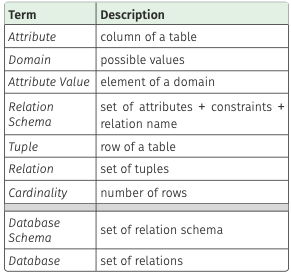
\includegraphics[width=0.85\linewidth]{1_relational_model.png}
    \begin{itemize}
      \item \underline{Relational Schema:} Defines a relation, specifies attributes (columns), data constraints, name 
      \begin{itemize}
        \item $R(A_1, A_2, \dots A_3)$: relation schema with name $R$ and $n$ attributes $A_1, A_2, \dots, A_n$
        \item Eg. \verb|Employees(id:INT, name:TEXT, dob:DATE)|
      \end{itemize}
      \item \underline{Domain:} Set of atomic values, including NULL
      \begin{itemize}
        \item $dom(A_i)$ = set of possible values for $A_i$
        \item $\forall$ value $v$ of attribute $A_i$, $v \in \{dom(A_i \cup \{null\})\}$
      \end{itemize}
    \end{itemize}

    \subsection{Keys}
    \begin{itemize}
      \item \textbf{Superkey:} Subset of attributes that UNIQUELY IDENTIFIES  a tuple in a relation
      \item \textbf{Key:} Superkey that is also MINIMAL (No proper subset of key is a superkey)
      \item \underline{Properties of Superkeys \& Keys:}
      \begin{enumerate}
        \item If (A,B,C) is DEFINITELY superkey $\rightarrow$ (A,B,C,D) is superkey
        \item If (A,B,C) is DEFINITELY key $\rightarrow$ (A,B,C) is superkey
        \item If (A,B) is DEFINITELY superkey $\rightarrow$ (A,B,C) is NOT a key
        \item If (A,B) is DEFINITELY key $\rightarrow$ possible (B,C,D) is also key
        \item Every relation has $\geq$ 1 superkey
      \end{enumerate}
      \item \textbf{Candidate Key:} Set of all keys of a given relation
      \item \textbf{Primary Key:} A selected candidate key (attributes CANNOT be NULL, is underlined in schema notation)
      \item \textbf{Foreign Key:} Subset of attributes of relation $R_1$ that refers to Primary Key of relation $R_2$
      \begin{itemize}
        \item $R_1$ is referencing relation, $R_2$ is referenced relation
        \item $R.sid \rightarrow S.id$: $R.sid$ is a FK referencing PK $id$ in $S$
        \item FK in $R_1$ must appear as PK in $R_2$ OR be NULL/tuple containing at least 1 NULL value
        \item A referencing relation can be a referenced relation for different foreign key $\vert$ Referencing relation \& referenced relation can be same relation
      \end{itemize}
    \end{itemize}
  \end{multicols*}
\end{document}
